\setcounter{section}{9}
\section{TP10 - Context-Free Languages (CFLs)}
{
\renewcommand{\thesubsubsection}{\thesubsection\alph{subsubsection}}
\begin{lemma}[Pumping lemma for CFLs] \label{lem:pumpCFL}
Given a context-free language $L \in \Sigma^*$,
\begin{equation*}
	\exists n \in \mathbb{N}^+ \colon \forall z, |z|\geq n \implies \exists u, v, w, x, y \in \Sigma^* \colon 
	\begin{cases}
		z=uvwxy\\
		|vwx| \leq n\\
		vx \neq \varepsilon \\
		\forall k \in \mathbb{N},\,u\,v^k\,w\,x^k\,y \in L
	\end{cases}
\end{equation*} 
\end{lemma}
\subsection{Exercise 1} \label{TP10_1}
This DPDA accepts by empty stack, and only works for $m \geq 1$.
\begin{center} 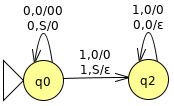
\includegraphics[scale=0.5]{TP10_1} \end{center}
It is hardly possible to make a DPDA that works for $m \geq 0$, since for $m \geq 1$ there is an absolute need to fill the stack with $0$s, but for $m=0$ it would be needed to have a spontaneous transition to a state that empties the stack.\\
One option is to consider a DPDA that accepts by empty stack in general, but also accepting by final state just for one state $q_0$.
\begin{center} 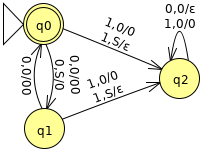
\includegraphics[scale=0.5]{TP10_2} \end{center}
Another option takes advantage of the fact programming languages generally represent strings with a null terminator at the end, which we will denote by $E$.
\begin{center} 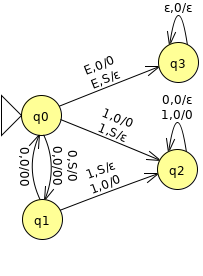
\includegraphics[scale=0.5]{TP10_3} \end{center}
\subsection{Exercise 2}
The PDA of \hyperref[TP09_1b]{9.1b} is non-deterministic because $\#\delta(q_0,\varepsilon,S)=3$.\\
The PDA of \hyperref[TP09_2]{9.2} is non-deterministic because $\#\delta(q_0,\varepsilon,A)=3$.\\
The PDA of \hyperref[TP09_3]{9.3} is non-deterministic because $\#\delta (q_0,\varepsilon, S)=4$.\\
All PDAs of \ref{TP10_1} are deterministic.
\subsection{Exercise 3}
All CFLs can be represented by a NPDA, but not by a DPDA.
\subsection{Exercise 4}
\begin{minipage}[c]{0.25\textwidth} \begin{alignat*}{2}
	S &\rightarrow A1B \\
	A &\rightarrow 0A\,|\,\varepsilon\\
	B &\rightarrow 0B\,|\,1B\,|\,\varepsilon
\end{alignat*} \end{minipage}%
\begin{minipage}[c]{0.25\textwidth} \begin{alignat*}{2}
	S &\rightarrow 1B\,|\,A1B \\
	A &\rightarrow 0A\,|\,0\\
	B &\rightarrow 0B\,|\,1B\,|\,\varepsilon
\end{alignat*} \end{minipage}%
\begin{minipage}[c]{0.25\textwidth} \begin{alignat*}{2}
	S &\rightarrow 1\,|\,1B\,|\,A1\,|\,A1B \\
	A &\rightarrow 0A\,|\,0\\
	B &\rightarrow 0\,|\,1\,|\,0B\,|\,1B
\end{alignat*} \end{minipage}%
\begin{minipage}[c]{0.25\textwidth} \begin{alignat*}{2}
	S &\rightarrow 1\,|\,1B\,|\,A1\,|\,AE_1 \\
	E_1 &\rightarrow 1B\\
	A &\rightarrow 0A\,|\,0\\
	B &\rightarrow 0\,|\,1\,|\,0B\,|\,1B
\end{alignat*} \end{minipage}
\begin{alignat*}{2}
	S &\rightarrow G_1\,|\,G_1B\,|\,AG_1\,|\,AE_1 \\
	E_1 &\rightarrow G_1B\\
	A &\rightarrow G_0A\,|\,G_0\\
	B &\rightarrow G_0\,|\,G_1\,|\,G_0B\,|\,G_1B\\
	G_0 &\rightarrow 0\\
	G_1 &\rightarrow 1
\end{alignat*}
\subsection{Exercise 5}
\begin{center}
\begin{minipage}[c]{0.3\textwidth} \begin{alignat*}{2}
	S &\rightarrow 0S00\,|\,0B0\,|\,B\\
	B &\rightarrow 11B22\,|\,12\,|\,C\\
	C &\rightarrow 0\,|\,\varepsilon
\end{alignat*} \end{minipage}%
\begin{minipage}[c]{0.3\textwidth} \begin{alignat*}{2}
	S &\rightarrow 0S00\,|\,0B0\,|\,B\\
	B &\rightarrow 11B22\,|\,12\,|\,0\,|\,\varepsilon
\end{alignat*} \end{minipage}%
\begin{minipage}[c]{0.4\textwidth} \begin{alignat*}{2}
	S &\rightarrow 0S00\,|\,00\,|\,0B0\,|\,B\,|\,\varepsilon\\
	B &\rightarrow 11B22\,|\,1122\,|\,12\,|\,0
\end{alignat*} \end{minipage}
\end{center}
\begin{center}
\begin{minipage}[c]{0.3\textwidth} \begin{alignat*}{2}
	S &\rightarrow 0E_1\,|\,00\,|\,0E_2\,|\,B\,|\,\varepsilon\\
	E_1 &\rightarrow S00\\
	E_2 &\rightarrow B0\\
	B &\rightarrow 11B22\,|\,1122\,|\,12\,|\,0
\end{alignat*} \end{minipage}%
\begin{minipage}[c]{0.3\textwidth} \begin{alignat*}{2}
	S &\rightarrow 0E_1\,|\,00\,|\,0E_2\,|\,B\,|\,\varepsilon\\
	E_1 &\rightarrow SE_3\\
	E_2 &\rightarrow B0\\
	E_3 &\rightarrow 00\\
	B &\rightarrow 1E_4\,|\,1E_5\,|\,12\,|\,0\\
	E_4 &\rightarrow 1E_6\\
	E_5 &\rightarrow 1E_7 \\
	E_6 &\rightarrow BE_7\\
	E_7 &\rightarrow 22\\
\end{alignat*} \end{minipage}%
\begin{minipage}[c]{0.4\textwidth} \begin{alignat*}{2}
	S &\rightarrow G_0E_1\,|\,G_0G_0\,|\,G_0E_2\,|\,B\,|\,\varepsilon\\
	E_1 &\rightarrow SE_3\\
	E_2 &\rightarrow BG_0\\
	E_3 &\rightarrow G_0G_0\\
	B &\rightarrow G_1E_4\,|\,G_1E_5\,|\,G_1G_2\,|\,G_0\\
	E_4 &\rightarrow G_1E_6\\
	E_5 &\rightarrow G_1E_7 \\
	E_6 &\rightarrow BE_7\\
	E_7 &\rightarrow G_2G_2\\
	G_0 &\rightarrow G_0\\
	G_1 &\rightarrow G_1\\
	G_2 &\rightarrow G_2
\end{alignat*} \end{minipage}
\end{center}
\subsection{Exercise 6}
\begin{theorem}
The language $L=\{a^nb^nc^i\,|\,n \leq i \leq 2n\}$ is not a CFL.
\end{theorem}
\begin{proof}
Assume by absurd that $L$ is a CFL. By the pumping lemma \eqref{lem:pumpCFL},
\begin{equation*}
	\exists n \in \mathbb{N}^+ \colon \forall z, |z|\geq n \implies \exists u, v, w, x, y \in \Sigma^* \colon 
	\begin{cases}
		z=uvwxy\\
		|vwx| \leq n\\
		vx \neq \varepsilon \\
		\forall k \in \mathbb{N},\,u\,v^k\,w\,x^k\,y \in L
	\end{cases}
\end{equation*}
Say we know the value of $n$. Consider now the string $z=a^nb^nc^{2n}$, which verifies $|z|=4n \geq n$. \\
Given that $|vwx|\leq n$, $vwx$ cannot simultaneously contain $a$'s and $c$'s:
\begin{itemize}
	\item If $vwx$ does not contain $c$'s, then it contains only $a$'s and $b$'s. By the pumping lemma, $uwy \in L$. Because $vx$ is not empty, $uwy$ has $2n$ $c$'s at the end, but either less than $n$ $a$'s, less than $n$ $b$'s or both.
	\item If $vwx$ does not contain $a$'s, then it contains only $b$'s and $c$'s. By the pumping lemma, $uv^2wx^2y \in L$. Because $vx$ is not empty, $uv^2wx^2y$ has $n$ $a$'s at the beginning, but either more than $n$ $b$'s, more than $2n$ $c$'s or both.
\end{itemize}
We have thus arrived at a contradiction in all cases, meaning we have proven the theorem correct.
\end{proof}
\subsection{Exercise 7}
\begin{theorem}
	$L=\{0^p\,|\,p \text{ is prime}\}$ is not a CFL.
\end{theorem}
\begin{proof}
Assume by absurd that $L$ is a CFL. By the pumping lemma \eqref{lem:pumpCFL},
\begin{equation*}
	\exists n \in \mathbb{N}^+ \colon \forall z, |z|\geq n \implies \exists u, v, w, x, y \in \Sigma^* \colon 
	\begin{cases}
		z=uvwxy\\
		|vwx| \leq n\\
		vx \neq \varepsilon \\
		\forall k \in \mathbb{N},\,u\,v^k\,w\,x^k\,y \in L
	\end{cases}
\end{equation*}
Say we know the value of $n$. Consider now the string $z=0^p$ where $p$ is the smallest prime $p\geq n$, which verifies $|z|=p \geq n$.\\
Then, $u$, $v$, $w$, $x$, $y$ are of the form
\begin{equation*}
	\begin{cases}
		u=0^a\\
		v=0^b\\
		w=0^c\\
		x=0^d\\
		y=0^e
	\end{cases}
\end{equation*}
where $b+c+d \leq n$ and $b+d \neq 0$.\\
By the pumping lemma, the number of strings $z\in L$ with length $|z|\leq s$ is $f(s)$.
Considering that $a$, $b$, $c$, $d$ and $e$ are constants,
\begin{alignat*}{2}
	a+bk+c+dk+e=s
	&\iff a+c+e+k(b+d)=0\\
	&\iff k           =\frac{s-a-c-e}{b+d}
\end{alignat*}
\begin{equation} \label{eq:TP10_7_1}
	f(s) \geq \left\lfloor \frac{s-a-c-e}{b+d} \right\rfloor \iff f(s) \gtrsim s
\end{equation}
Given the definition of $f(s)$, it is trivially equal to the prime counting function: $f(s)=\pi(s)$.\\
By the prime number theorem,
\begin{equation} \label{eq:TP10_7_2}
	f(s) = \pi(s) \iff f(s) \sim \frac{s}{\ln{s}}
\end{equation}
Equations \eqref{eq:TP10_7_1} and \eqref{eq:TP10_7_2} give rise to a contradiction. We have thus proven the theorem.
\end{proof}
\pagebreak
\subsection{Exercise 8}
\begin{theorem}
The language $L=\{0^i1^{i^2}\}$ is not a CFL.
\end{theorem}
\begin{proof}
Assume by absurd that $L$ is a CFL. By the pumping lemma \eqref{lem:pumpCFL},
\begin{equation*}
	\exists n \in \mathbb{N}^+ \colon \forall z, |z|\geq n \implies \exists u, v, w, x, y \in \Sigma^* \colon 
	\begin{cases}
		z=uvwxy\\
		|vwx| \leq n\\
		vx \neq \varepsilon \\
		\forall k \in \mathbb{N},\,u\,v^k\,w\,x^k\,y \in L
	\end{cases}
\end{equation*}
Say we know the value of $n$. Consider now the string $z=0^n1^{n^2}$, which verifies $|z|=n+n^2 \geq n$. \\
Given that $|vwx|\leq n$, $vwx$ either contains: only $0$'s; only $1$'s; $v$ or $x$ have $0$'s and $1$'s; v has only $0$'s and $x$ only $1$'s:
\begin{itemize}
	\item $vwx=0^a$, $1 \leq a \leq n$. Because $vx$ is not empty, $uwy$ has $n^2$ $1$'s at the end but less than $n$ $0$'s at the beginning.
	\item $vwx=1^a$, $1 \leq a \leq n$. Because $vx$ is not empty, $uwy$ has $n$ $0$'s at the beginning but less than $n^2$ $1$'s at the end.
	\item $v=0^a1^b \vee x=0^a1^b$, $a,b \geq 1$, $a+b \leq n$. This means $uv^2wx^2y$ is no longer of the form $0^*1^*$ because there is alternance of $0$'s and $1$'s.
	\item $v=0^a$, $x=1^b$, $a,b \geq 1$, $a+b \leq n$. This means a string $z=uv^kwx^ky$ has
	\begin{alignat}{2}
		\label{eq:num0s} \# 0 &= n+a(k-1)\\
		\label{eq:num1s} \# 1 &= n^2+b(k-1)
	\end{alignat}
	Let $s$ be the size of the string, and $r=\#1/\#0$ the ratio of $1$'s to $0$'s. Considering $n$, $a$ and $b$ constants, for $k$ assimptotically larger than $n$, we have
	\begin{alignat}{3}
		\label{eq:sizerel0} s &= n^2+n+a(k-1)+b(k-1)         &&\sim k        &&\text{ by \eqref{eq:num0s} and \eqref{eq:num1s}} \\
		r &= \frac{n^2+b(k-1)}{n+a(k-1)} &&\sim b/a      &&\text{ by \eqref{eq:num0s} and \eqref{eq:num1s}} \\
		\label{eq:sizerel} s &= n^2+n    &&\sim n^2      &&\text{ by the definition of the language}\\
		r &= n \sim \sqrt{s}             &&\sim \sqrt{k} &&\text{ by  the definition of the language, \eqref{eq:sizerel} and \eqref{eq:sizerel0}}
	\end{alignat}
	which gives rise to the false statement $b/a \sim \sqrt{k}$, given $b/a$ is a constant but $k$ is assimptotically large.
\end{itemize}
We have thus arrived at a contradiction in all cases, meaning we have proven the theorem correct.
\end{proof}
\subsection{Exercise 9}
\textcolor{red}{Incomplete}\\
This question demands a lot of effort for the relatively low return, given it asks one to try to make a proof we know at start will not be successful.
\subsection{Exercise 10}
\subsubsection{Item a}
\begin{alignat*}{2}
	\inter(00,111)=\{&00111,\\
	&01011,\\
	&01101,\\
	&01110,\\
	&10011,\\
	&10101,\\
	&10110,\\
	&11001,\\
	&11010,\\
	&11100\}
\end{alignat*}
\subsubsection{Item b}
$L_1=L(0^*)$ and $L_2=\{0^n1^n\,|\,n\geq 0\}$.
\begin{equation*}
	\inter(L_1,L_2)=\{w=0^a1z\,|\,z \in \{0,1\}^* \wedge \#1\geq a\}
\end{equation*}
\subsubsection{Item c}
\begin{theorem}
	If $L_1$ and $L_2$ are regular languages, then $\inter(L_1,L_2)$ is a regular language.
\end{theorem}
\begin{proof}
Consider $D_1$, $D_2$ and $D$ as the DFAs of $L_1$, $L_2$ and $\inter(L_1,L_2)$ respectively. $D$ is constructed from $D_1$ and $D_2$ as follows:
\begin{enumerate}
	\item If $q_1$ and $q_2$ are the initial states of $D_1$ and $D_2$, then $(q_1,q_2)$ is the initial state of $D$.
	\item If $\delta_1(q,a)=p$, then $\forall r \in Q_2, \delta((q,r),a)=(p,r)$.
	\item If $\delta_2(q,a)=p$, then $\forall r \in Q_1, \delta((r,q),a)=(r,p)$.
	\item If $q_1\in F_1$ and $q_2 \in F_2$, then $(q_1,q_2) \in F$.
\end{enumerate}
This algorithm works, thus proving the theorem.
\end{proof}
\subsubsection{Item d}
\begin{theorem}
	If $L$ is a CFL and $R$ a RE, then $\inter(L,R)$ is a CFL.
\end{theorem}
\begin{proof}
Consider $D$ as the DFA of $R$, and $P_L$ and $P$ as the PDAs of $L$ and $\inter(L,R)$ respectively. $P$ is constructed from $P_L$ and $D$ as follows:
\begin{enumerate}
	\item If $q_L$ and $q_R$ are the initial states of $P_L$ and $D$, then $(q_L, q_R)$ is the initial state of $P$.
	\item The start symbol of $P$ is the same as $P_L$.
	\item If $\delta_L(q,a,s)=\{(p_1,\gamma_1),(p_2,\gamma_2),...\}$ then $\forall r \in Q_R, \delta((q,r),a,s)=\{((p_1,r),\gamma_1),((p_2,r),\gamma_2),...\}$.
	\item if $\delta_R(q,a)=p$, then $\forall r \in Q_L, \forall s \in \Gamma, \delta((r,q),a,s)=\{((r,p),s)\}$.
\end{enumerate}
This algorithm works, thus proving the theorem.
\end{proof}
\subsection{Exercise 11}
\begin{theorem}
In a grammar in the Chomsky Normal Form, all analysis trees of length n have 2n-1 inner nodes.
\end{theorem}
\begin{proof}
\textcolor{red}{Incomplete}
\end{proof}
}
